% Validity Ladder, Behavior Research Methods submission draft.
% Build: tectonic -X compile main.tex   (BibTeX runs automatically; apacite in natbibapa mode)
%
% Conventions used in the source (read before editing):
%   - One sentence per line.
%   - A line that carries a number ends with "% R: file.csv[; file.csv]" naming the receipt in
%     analysis/brm/ (or analysis_brm/*.md where noted). scripts/86_receipts.py parses these tags
%     into the receipts table (supplement S2) and checks each number against its file.
%   - \PATRICK{...} marks text the author has still to write. It prints as a red bracket.
%   - \CHECK{...} marks a fact still to confirm before submission.
\documentclass[man,12pt,floatsintext,natbib]{apa7}
\usepackage[natbibapa]{apacite}
\usepackage{amsmath,amssymb}
\usepackage{booktabs}
\usepackage{array}
\usepackage{graphicx}
\usepackage{xcolor}
\usepackage{catchfile}
\usepackage{placeins}
% The abstract is read into a macro: apa7 cannot take \input inside \abstract.
\CatchFileDef{\abstracttext}{sections/00_abstract.tex}{}
\graphicspath{{figures/}}

\newcommand{\PATRICK}[1]{\textcolor{red}{\textbf{[PATRICK:} #1\textbf{]}}}
\newcommand{\CHECK}[1]{\textcolor{orange}{\textbf{[CHECK:} #1\textbf{]}}}
% Verdict words at level 2 are the rule's output; set them in small caps so they read as labels.
\newcommand{\vd}[1]{\textsc{#1}}
% Table notes as an environment (apa7's \tablenote is a one-argument command that needs threeparttable).
\newenvironment{tabnote}{\par\vspace{2pt}\small\raggedright}{\par}

\title{A Validity Ladder for LLM-Simulated Populations}
\shorttitle{Validity Ladder for Simulated Populations}
\authorsnames{Patrick Keough}
\authorsaffiliations{Independent researcher}
\leftheader{Keough}
\authornote{
  % ORCID: paste the real iD and uncomment the next line.
  % \addORCIDlink{Patrick Keough}{0000-0000-0000-0000}

  Data, code and every receipt file are at
  \url{https://github.com/pskeough/A-Validity-Ladder-for-LLM-Simulated-Populations}. The Supplement is \texttt{paper\_brm/manuscript/supplement/supplement.pdf} in the same repository.

  Correspondence concerning this article should be addressed to Patrick Keough, Email: pskeough@gmail.com
}

\abstract{\abstracttext}
\keywords{silicon samples, large language models, simulated participants, validity, measurement invariance, PHQ-8, NHANES}

\begin{document}
% APA 7: "et al." from the first citation for three or more authors.
\shortcites{argyle2023outofone,bisbee2024synthetic,santurkar2023whose,dominguezolmedo2024questioning,park2024diminished,wang2025misportray,meister2025distributional,ma2025fidelity,wang2025sociobench,cao2025specializing,yu2025surveys,wang2024patientpsi,zack2024gpt4,pfohl2024toolbox,kuo2026synthetic,ballyk2026privacy,greene2026psychiatrist,chassat2026valid,desai2026validating,kim2026ier,hussain2024tutorial,duan2025macbehaviour,dillion2023replace,aher2023simulate,horton2023homosilicus,harding2024cannot,grossmann2023transformation,anthis2025position,tjuatja2024biases,sarstedt2024silicon,hamalainen2023hci,boelaert2025machinebias,rossi2024problems,binz2025centaur,serapiogarcia2025personality,pellert2024psychometrics,suhr2025personality,peereboom2025phantoms,hoang2026psibench,borsboom2004concept,lundberg2021estimand,aera2014standards,kroenke2001phq9,kroenke2009phq8,kroenke2010phqsads,lowe2004monitoring,wu2020equivalency,patel2019phq9,cintron2023intersectional,borgogna2021sexuality,keum2018phq9,villarrealzegarra2019invariance,perlis2025clinical,spitzer2006gad7,bush1998auditc,blevins2015pcl5,johnson2013nhanes,johnson2014nhanes,chen2018nhanes,akinbami2022nhanes,brody2018depression,drasgow1985appropriateness,magis2012lzstar,cronbach1972dependability,maccallum1996power,savalei2024rmsea,jorgensen2018permutation,raowuyue1992resampling,norman2003half,vancalster2019calibration,lakens2018tutorial,fda2026bioequivalence,anes2016timeseries,jiang2024personallm,toubia2025twin2k,suh2025subpop,huang2025uncertainty,peng2025funhouse,hullman2026validating,wang2026substitutability,petrov2024limited,jiang2023mistral,mercer2025hexaco,davern2024gss,bisbee2024data,argyle2023data}
% apacite prints APA 6 "doi:" and "Retrieved from" forms; these give APA 7 output.
\renewcommand{\doiprefix}{https://doi.org/\ignorespaces}
\renewcommand{\BRetrievedFrom}{}
\maketitle

% Section 1. Introduction.

Behavioral researchers now prompt large language models (LLMs) with demographic personas and treat the answers as \emph{silicon samples}.
\citet{argyle2023outofone} used such samples to reproduce vote choice and opinion by group, \citet{park2024diminished} used them to replicate classic experiments, and \citet{lin2026simulators} describes their use in piloting instruments before fielding them.
A simulated sample costs little, reaches groups that are hard to recruit, and can be rerun whenever the design changes.
Each of these uses assumes that the simulated sample stands in for a real one in the respect the study measures.

That assumption is checked unevenly.
Across eight social science journals, \citet{desai2026validating} found validation practice in LLM studies ``inconsistent and limited.''
\citet{park2024diminished} found GPT-3.5 answering with almost no variation where people vary, and \citet{bisbee2024synthetic} found synthetic opinion distributions narrower than the survey distributions they imitate.
\citet{wang2025misportray} showed that LLMs standing in for participants can misportray and flatten identity groups, and \citet{dominguezolmedo2024questioning} found that models' survey answers trend toward uniform randomness once ordering and labeling biases are adjusted for.
\citet{sarstedt2024silicon} set out guidelines for silicon samples in consumer research, and \citet{lin2026workflow} proposed a workflow in which the evidence a study needs rises with its claim, setting correspondence with a population's means, variance, scale structure and correlations as targets without a test attached to each.

One persona from the corpus analyzed here shows what reading individual answers misses.
Prompted as a single Black woman on Medicaid with a household income under \$35,000, GPT-4o-mini returns a PHQ-8 total of 8 on its first draw, a plausible answer in the mild band. % R: 85_worked_case.csv
Over thirty draws the same prompt averages 10.3, and adults in the National Health and Nutrition Examination Survey (NHANES) who share her race, sex, income and marital status average 4.7. % R: 85_worked_case.csv
None of her single answers shows that the simulated population she belongs to sits well above the real one.

We propose the validity ladder (Figure~\ref{fig:ladder}), which supplies a statistic, a pass rule and a human reference for each use, following the view in validity theory that each interpretation and use of a score needs its own evidence \citep{messick1995validity,kane2013validating,lin2026constructs}.
A gate measures how many repeated draws make a persona's score precise enough to read.
Above the gate, level 1 tests whether a single draw is an answer pattern a person could give, and level 2 tests whether gaps between groups match the population's.
Level 3 tests whether the population level matches, and level 4 tests whether the items relate to one another as they do in people.
A simulated sample supports only the claims whose rungs it has passed, and the rules are released as code.

In the worked example, the ladder is applied to PHQ-8 depression assessments that four language models produced as demographic personas \citep{keough2026plausible}, read against a national health survey.
Controls built from real survey respondents then test whether the ladder passes real people and catches failures planted at known sizes, a test any check on simulated samples has to pass before its verdicts on models carry weight.
The ladder is then applied to ten releases by other authors, ranging from silicon samples and digital twins to a model fine-tuned on survey answers \citep{suh2025subpop} and a personality inventory.
Together the three parts ask whether the ladder separates samples that stand in for people from samples that do not, on instruments and designs it was not built around.
The next section sets out each rung, the use it serves and what a study needs to run it.

% Section 2. The validity ladder. Full specification: Supplement S7 and paper_brm/LADDER_SPEC.md.

\section{The Validity Ladder}
\label{sec:ladder}

Whether a simulated sample resembles people breaks into several questions.
Each use of the sample is a separate inference from the model's answers to a population, and each can hold or fail on its own.
Reading a persona's score, treating one answer as a case, comparing groups, estimating a group's level and scoring a scale each rest on a different property of the sample.
The validity ladder names these uses, pairs each with the property it depends on and a test against human data, and orders them from narrow to broad, beginning with a gate that tests whether a score is stable enough to read.
In these terms, a researcher who prompts a language model with personas and collects its answers to a fixed instrument has a simulated sample.
The instrument may be a multi-item scale, a single survey item or an opinion question.
Each call to the model returns one draw, and each persona under one model and one prompt framing forms a cell of $k$ draws whose average is the persona mean.

The rungs differ in what they need (Figure~\ref{fig:ladder}).
Repeated draws of each persona are enough for the gate.
Levels 1 and 4 require a multi-item scale and individual human answers on it, and levels 2 and 3 require personas built on attributes the reference records and a reference that measures the resulting groups precisely.
Where a study cannot meet a rung's requirements, that rung is not run and its claims are not made.
Verdicts are given per model, because a pooled verdict can hide errors running in opposite directions.
Passing a test means it found no failure at the precision the data allow, and a test the reference is too imprecise to support is recorded as not read.
Only the gate is a prerequisite, and a failure at one level leaves the others to run.
The gate sets $k$ for levels 2 and 3.
A group comparison of a multi-item total also assumes that the scale measures the same construct in each group, and a pass at level 2 or 3 on a total is valid only beside a pass on the invariance rule of level 4.
All pass rules and thresholds serve as defaults a user may change.
Supplement S7 gives the full specification.

\begin{figure}[!ht]
\input{figures/fig1_ladder_caption}
{\centering\includegraphics[width=\linewidth]{fig1_ladder.pdf}\par}
\input{figures/fig1_ladder_note}
\end{figure}
\FloatBarrier

\subsection{Gate: Regeneration Stability}
\label{sec:gate-method}

Two calls to a model with the same persona prompt rarely return the same answer, and a study that reads one generation as a persona's answer reads the persona's score plus noise.
The gate asks how many draws must be averaged before that noise is small enough for the score to be read.
Following a generalizability study \citep{cronbach1972dependability,brennan2001gtheory}, the variation splits into $\sigma^2_p$, the spread between personas, and $\sigma^2_r$, the spread among draws of one persona.
Averaging $k$ draws gives a standard error and a dependability of
\begin{equation}
\mathrm{SE}(k) = \sqrt{\sigma^2_r / k}, \qquad \phi(k) = \frac{\sigma^2_p}{\sigma^2_p + \sigma^2_r / k}.
\label{eq:phi}
\end{equation}
Means of $k$ draws may be read once $\mathrm{SE}(k)$ falls to 0.25 reference standard deviations in each prompt framing, and the recommended $k$ takes it to 0.125.
Single draws may be read only if the draw-to-draw standard deviation is itself no larger than 0.25 reference standard deviations.
Dependability is reported beside every verdict and required ($\phi \ge .80$) only for studies that compare or rank individual personas.
Real demographic cells differ little, and a faithful simulator shows the same small differences.
Passing supports reading the $k$-draw mean as the model's answer for that persona, leaving the correctness of that answer to the levels above, and failing rules out persona-level readings until more draws are averaged.

\subsection{Level 1: Individual Coherence}
\label{sec:l1-method}

Exemplar vignettes, screener test items and synthetic respondents treat single draws as individual cases.
Real people with the same total answer in different patterns, most endorsing the common items before the rare ones and a minority answering in unusual ways, while a simulator can return each total in the same textbook pattern.
Level 1 fits a graded response model \citep{samejima1969graded} to the human reference with survey weights and gives every respondent and every draw the standardized person-fit statistic $l_z^*$ \citep{drasgow1985appropriateness,snijders2001personfit,sinharay2016personfit}, low for an unusual pattern and high for an unusually regular one.
Each draw is set against real respondents with the same total.
The \emph{misfit ratio} divides the share of draws more unusual than 95\% of matched respondents by the 5\% expected, and the \emph{overfit ratio} does the same for draws more regular than 95\% of them.
In a real population both equal 1.
A model passes in a framing when the 90\% intervals of both ratios fall between $1/\tau$ and $\tau$, where $\tau$ is the smallest of 1.5, 2 and 3 that covers every clear departure from 1 shown by real subgroups of the reference, with a floor of 1.5 set by the controls.
A model with too few patterns in both tails is \emph{compressed}.
Passing supports single draws as individual cases, and a compressed failure rules out any use resting on the spread of real presentations.

\subsection{Level 2: Subgroup Fidelity}
\label{sec:l2-method}

Many persona studies compare groups, reporting an income gradient in a symptom score or a partisan gap in an attitude.
Level 2 asks whether the gap between two groups has the population's size and direction.
The simulated gap $g$ compares personas that differ on one attribute and match on the rest, and the population gap $\gamma$ is computed the same way among people in the reference who match on the other attributes.
Level 2 reads the ratio $\rho = g/\gamma$, where 1 reproduces the population gap, 2 doubles it, 0 erases it and a negative ratio reverses it, with a Fieller interval \citep{fieller1954interval}.
The contrasts tested together on one model form its family, and each interval is widened by a Bonferroni correction over the family.

A contrast is \vd{kept} when its whole interval lies between 0.75 and 1.25, placing the simulated gap within a quarter of the real gap's size.
A contrast is \vd{not kept} when the interval lies wholly outside that range and \vd{unresolved} when it overlaps it.
A contrast that is not kept is named by its ratio, with ratios above 1.25 steepened, from 0.25 to 0.75 attenuated, near zero missing and negative reversed.
A contrast is \vd{not read} in two cases.
The first is when the reference cannot tell the contrast's population gap from zero.
The second is when the reference measures the gap too imprecisely for any simulated gap to be read kept, unless the contrast is already clearly not kept.
A model passes level 2 when at least one contrast is read and every contrast read is kept, fails when any is not kept, and is otherwise unresolved.
A pass supports reading the size and direction of group differences from the sample, leaving either group's level to level 3, and a failure rules out the group comparisons it names.

The second case depends on the reference alone and can be checked before any model is run, a check the ladder calls step 0.
A contrast is certifiable when a faithful simulator with no sampling noise, whose gap equals the population gap, would be read kept at the family's Bonferroni level (Supplement S7).
When a family has no certifiable contrast and its verdict is unresolved, it is reported as \vd{reference cannot certify}, and passes and failures stay as they are.
Run on a planned reference, step 0 lists the gaps a study could certify, and a researcher can enlarge the reference or narrow the claims before generating.

\subsection{Level 3: Population Calibration}
\label{sec:l3-method}

Level 3 serves studies that use a simulated sample in place of a survey to estimate a group's level, such as the prevalence of a condition or the share agreeing with a policy.
A persona grid holds one persona for each combination of attributes, while a real group contains those combinations in unequal shares.
Each persona cell $c$ in a group $G$ is therefore weighted by its share $p_c$ of that group in the reference, and the residual for the group is
\begin{equation}
R_G = \sum_{c \in G} p_c\,(s_c - y_c),
\end{equation}
where $s_c$ is the persona mean and $y_c$ the mean of real respondents who match that persona \citep{holtsmith1979poststrat}.
Draw error within cells and a design-based jackknife of the survey together give its interval.
A group row passes at tolerance $\delta$ when its 90\% interval lies within $\pm\delta$, by two one-sided tests \citep{schuirmann1987tost,lakens2018tutorial}, with $\delta$ named by the researcher as the smallest difference that matters for the use.
Half a reference standard deviation is the default and 0.2 standard deviations the strict alternative.
Because a correct mean can hide a wrong prevalence, the share at or above the instrument's cut point enters as a second row, and every row must pass.
A pass supports using the simulated level in place of the group's level, within $\delta$, for the prompt, persona grid and survey period tested.

\subsection{Level 4: Structural Fidelity}
\label{sec:l4-method}

Level 4 serves studies that sum the items of a scale into one total and compare groups on it.
In people the items of a validated scale rise and fall together, and the total measures one thing.
A simulator can return plausible totals whose items do not.
Level 4 treats the draws of one model in one framing as one population, resampled by persona, and fits a one-factor model to the polychoric item correlations \citep{olsson1979polychoric}.
The fit is checked against three rules, numbered as in the full specification in Supplement S7.
Rule R1, a general factor, requires every loading to be at least .30 and the first eigenvalue at least three times the second, or the reference's own value where the reference falls short.
Rule R2, loadings like people's, requires Tucker's congruence of at least .95 \citep{lorenzoseva2006congruence} and a root mean square loading difference of at most .10, each at the conservative end of its 90\% interval.
Rule R4, the same scale in every group, requires the factor to be invariant across the groups the reference records wherever it is in people, read on the RMSEA of each invariance step \citep{savalei2024rmsea} against a margin of .08.
A model passes level 4 when it passes all three rules in every framing.
R1 and R2 support scoring the total as one score with item weights like people's, and R4 adds that a group comparison of the total means what it means in people.
The specification's R3, whether the factor holds among draws of one persona, is a diagnostic and does not decide the verdict.

% Section 3.1. Worked example: data. Prompts and row provenance are in Supplement S1 and S3.

\section{Worked Example}
\label{sec:data}

\subsection{Data}

The worked example uses the corpus of \citet{keough2026plausible}, in which language models answered the eight-item Patient Health Questionnaire depression scale (PHQ-8; \citealp{kroenke2009phq8}) as demographic personas.
Four models, GPT-4o-mini, Gemini-3-Flash, DeepSeek-V3 and GLM-4.7, generated the corpus through OpenRouter between 28 December 2025 and 11 January 2026, at the provider's default decoding. % R: corpus_v3_provenance.csv
The persona grid crosses race (Asian, Black, Hispanic, multiracial, White), gender identity (cisgender and transgender women and men), income (three levels, stated as a dollar-and-insurance label from ``Low (<\$35k, Medicaid)'' to ``High (>\$250k, Concierge)'') and relationship status (married, single), for 120 personas.
Each persona answered 30 times under each of two framings, one listing its attributes as fields (clinical) and one giving them as a first-person self-description (narrative).
A shared system prompt cast the model as a ``Clinical Simulation Engine'' answering from ``the statistical likelihood of symptoms for this specific demographic intersection in the US population''.
The corpus holds 28,800 assessments, of which 28,799 have a valid PHQ-8, and Supplements S1 and S3 give the prompts and the provenance of every row. % R: corpus_v3_provenance.csv; l1_personfit_main.csv

The population reference is the 36,274 adults in NHANES 2005--2018 who answered all eight PHQ-8 items, analyzed with the survey's weights and design \citep{johnson2013nhanes,chen2018nhanes,nchs2018analytic}. % R: l1_nhanes_sample_flow.csv; analysis_brm/L4.md
Income is the ratio of family income to the poverty line, banded below 1.3, from 1.3 to 3.5, and above 3.5, and each persona's income label is mapped to one band.
Forty-eight of the 120 personas have a matching group in the survey.
NHANES records sex rather than gender identity and does not identify multiracial adults on their own, and transgender and multiracial personas therefore enter only levels 1 and 4, which read the whole simulated population.
NHANES 2021--2023 and other reference choices are sensitivity analyses in Supplement S3.

The NHANES standard deviation of the PHQ-8 total sets the gate tolerances at 0.98 and 0.49 points and the default level-3 tolerance at about 2 points. % R: gate_dstudy.csv
No NHANES subgroup by sex, race and ethnicity, income or survey cycle departs from 1 by more than a factor of 1.36 at level 1, or 1.27 at the near end of its interval, and level 1 uses $\tau = 1.5$. % R: l1_personfit_tolerance.csv
Level 2 reads seven contrasts for each model, the sex gap, three income gaps and three racial gaps, with Bonferroni-adjusted 98.6\% intervals.
Levels 2 and 3 use the mean of all 30 draws of each persona, more than the gate requires for any model, and level 4 tests invariance across sex, race and income.

% Section 3.2. Worked example: results. The claims table moved to Supplement S4.8 in the 4 Oct 2026 condense pass.

\subsection{Results}
\label{sec:results}

\begin{table}[!ht]
\centering
\caption{Ladder Verdicts per Model in the Worked Example}
\label{tab:verdicts}
\small
\newcolumntype{P}[1]{>{\raggedright\arraybackslash}p{#1}}
\begin{tabular}{@{}lP{2.1cm}P{2.3cm}P{1.9cm}P{1.9cm}P{2.5cm}@{}}
\toprule
Model & Gate: draws needed (min.\ / rec.) & Level 1: single draws & Level 2: income gap ratio & Level 3: overall residual & Level 4: structure \\
\midrule
DeepSeek-V3 & Pass (3 / 9) & Fail, compressed & Fail, 1.91 & Fail, +4.6 & Fail, no general factor \\ % R: gate_dstudy.csv; l2_headline.csv; 80d_headline.csv
Gemini-3-Flash & Pass (3 / 10) & Fail, compressed & Fail, 5.07 & Fail, +2.6 & Fail, loadings (R2) and invariance (R4) \\ % R: gate_dstudy.csv; l2_headline.csv; 80d_headline.csv
GPT-4o-mini & Pass (4 / 13) & Fail, compressed & Fail, 2.16 & Fail, +4.7 & Fail, no general factor \\ % R: gate_dstudy.csv; l2_headline.csv; 80d_headline.csv
GLM-4.7 & Pass (6 / 21) & Fail, too few atypical & Fail, 5.03 & Fail, +2.1 & Fail, loadings (R2) and invariance (R4) \\ % R: gate_dstudy.csv; l2_headline.csv; 80d_headline.csv
\bottomrule
\end{tabular}
\vspace{4pt}
\begin{tabnote}
\textit{Note.} Gate: draws needed for a persona mean's standard error to reach 0.25 (minimum) and 0.125 (recommended) NHANES standard deviations, the larger of the two framings. Level 2: ratio of the simulated to the standardized NHANES gap between low- and high-income personas, where 1 reproduces the gap. Level 3: post-stratified simulated minus NHANES mean PHQ-8, in points. Level 4: R2, loadings stronger than people's; R4, the factor differs across income where it does not in NHANES. Full per-level tables are in Supplement S4.
\end{tabnote}
\end{table}
\FloatBarrier

All four models pass the gate and fail every level above it (Table~\ref{tab:verdicts}), and Figure~\ref{fig:panels} shows what each failure looks like.

\begin{figure}[tp]
% Figure 2 title. Drawn by scripts/84e_fig2_ladder_panels.py from analysis/brm/gate_dstudy.csv,
% l1_summary.csv, 80d_headline.csv and l4_structure.csv. Every level-2 interval is in Supplement Figure S1.
\caption{Failures of the Four Models in the Worked Example}
\label{fig:panels}

{\centering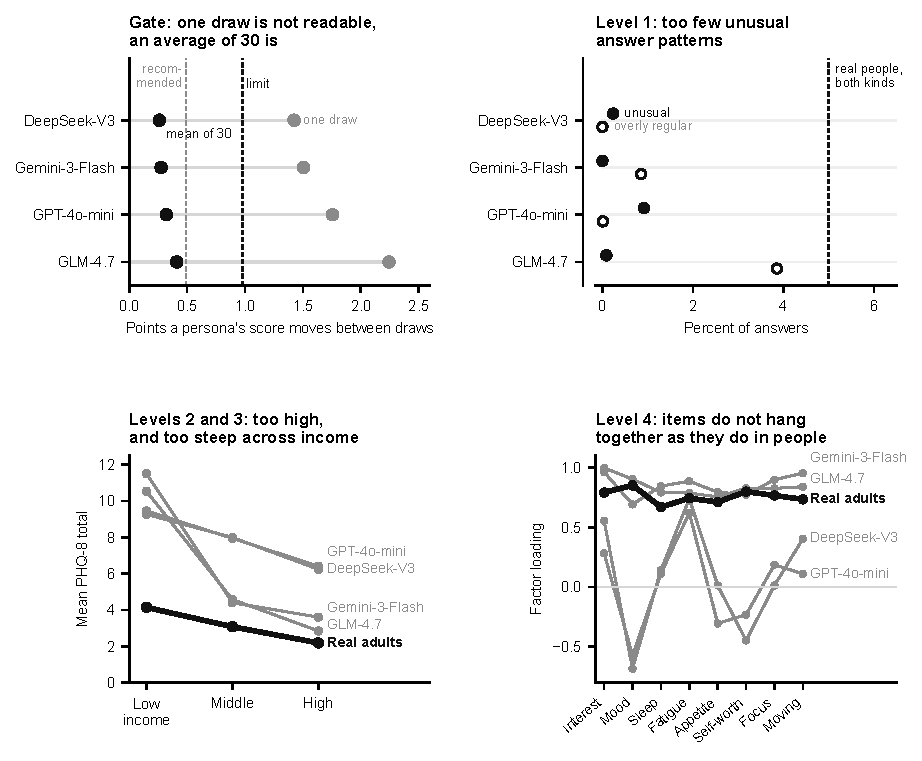
\includegraphics[width=\linewidth]{fig2_ladder_panels.pdf}\par}
% Figure 2 note (below the figure): how to read each panel.
\figurenote{Gate: how far a persona's PHQ-8 total moves between draws, for one draw (the draw standard deviation, larger framing) and for the mean of 30 (its standard error), against the gate's limit of 0.98 points and recommended level of 0.49. % R: gate_dstudy.csv
Level 1: percent of draws more unusual (filled) or more regular (open) than 95\% of NHANES adults with the same total, both framings, where real people give 5\% of each.
Levels 2 and 3: post-stratified mean PHQ-8 total in each income band.
Level 4: loading of each PHQ-8 item on a single factor in the narrative framing, where a loading near 1 means the item rises and falls with the rest of the scale and a loading near 0 or below means it does not. DeepSeek-V3 and GPT-4o-mini have no general factor, and Gemini-3-Flash and GLM-4.7 follow the human pattern with loadings stronger than people's.
Every level-2 interval is in Supplement Figure S1.}

\end{figure}

\paragraph{Gate.}
No model can be read from a single draw, and two draws of one persona fall in different PHQ-8 severity bands 32.2\% to 35.2\% of the time across the two framings. % R: gate_bandflip_summary.csv
Averages of a few draws are stable enough to read, with the minimum rule needing 3 to 6 draws per persona. % R: gate_dstudy.csv
Setting the temperature to 0 narrows the spread of draws without separating personas any better (Supplement S1.7), and averaging remains the way to read a persona's score.

\paragraph{Level 1.}
No model passes level 1 in either framing, at any tolerance up to 3 or at temperature 0 (Supplement S4). % R: l1_personfit_verdicts_tau.csv; 96_decoding_l1.csv
Where 5\% of NHANES adults give an unusual answer pattern for their total, the models give 0.0\% to 1.0\%, and three of the four are compressed in both tails. % R: l1_summary.csv
A vignette bank or a screener test set drawn from these samples would miss almost all of the unusual presentations that one in twenty real respondents give.

\paragraph{Level 2.}
Every model fails level 2 on income, steepening the gap between low- and high-income personas to 1.91 to 5.07 times the population gap (Supplement Figure S1). % R: l2_headline.csv
We read the size of that ratio as partly a product of how the persona's income label is matched to the survey, although every model still fails on an income contrast when income is matched on the label's dollar amount (Supplement S3). % R: l2_verdicts.csv
On the sex gap the models disagree, two shrinking it, one doubling it and one unresolved, and pooled over the four models the ratio is 0.97, a near match built from errors in opposite directions. % R: l2_headline.csv
No racial contrast is kept, and NHANES measures the racial gaps among matched adults too loosely to certify any simulator. % R: l2_stop.csv; l2_headline.csv
None of these samples can estimate how depression differs by income, sex or race, and a study of the racial gaps needs a larger or more targeted reference before the ladder can read them.

\paragraph{Level 3.}
Every simulated population is more depressed than NHANES, by 2.1 to 4.7 points overall, and every group in every model sits above its real counterpart. % R: 80d_headline.csv; 80d_pass_counts.csv
The excess is largest in the low-income band, where 55.5\% of simulated respondents score 10 or more against 13.6\% of real adults, and it holds under all eight reference specifications (Supplement S3). % R: 80d_headline.csv; 89_l3_spec_range_summary.csv
Prevalence errs in a different pattern from the mean, and DeepSeek-V3's overall prevalence looks correct only because a low-income excess cancels shortfalls elsewhere. % R: 80d_model_verdicts.csv
Read as a stand-in for a survey, these samples would overstate depression for every group, most of all among low-income adults.

\paragraph{Level 4.}
DeepSeek-V3 and GPT-4o-mini have no general factor, and their PHQ-8 total cannot be scored as one measure. % R: l4_structure.csv
Gemini-3-Flash and GLM-4.7 have a factor with the human pattern of loadings, but loadings stronger than people's and a structure that changes across income where it holds in NHANES. % R: l4_structure.csv; l4_r2_size.csv; l4_invariance.csv
Their factor is built from differences between persona means, and draws of one persona share none, the same uniformity within personas that level 1 found (Supplement S4). % R: l4_between_within.csv

\paragraph{Summary.}
Read one at a time, every model's answers look like believable patients, and averages of a few draws are stable enough to read.
The introduction's persona shows the pattern on one case, with each of her draws plausible, the set less varied than people at her severity, and her mean well above matched NHANES adults in both framings. % R: 85_worked_case.csv
A researcher who checked this sample only by reading its answers or by the stability of its scores would have accepted it.
Checks of the kind used to report algorithmic fidelity would have looked reassuring as well.
Across the 48 matched persona cells the models' persona means correlate with the means of matching NHANES adults at .72 to .82, and every model gives at least five of the seven level-2 gaps the population's direction (Supplement S4.9). % R: 99_naive_baseline.csv
Neither a correlation nor a count of gap directions registers that every group is too depressed or that the income gradient is up to five times too steep.
The ladder fails it at every level above the gate, finding its answers too uniform, its income gradient too steep, every group too depressed and its total without the structure the PHQ-8 has in people.

\paragraph{Using the verdicts.}
We read the verdicts as a list of supported and ruled-out uses for a researcher holding this corpus.
Persona means can be read after a few draws, while single answers as cases, group comparisons, population estimates and scale totals are all ruled out for these samples.
The verdicts hold for these four models under this prompt family, and a new model, prompt or persona wording calls for the ladder to be run again.
A prompt control that asked each model to answer as the person described did not remove the excess at level 3, although it left unchanged the income labels, which paired a dollar amount with an insurance type (Supplement S1.6). % R: ../prompt_control_results.csv

% Section 4. Controls. Dose detection and calibration details are in Supplement S5.

\section{Controls}
\label{sec:controls}

With every model failing every rung above the gate, the ladder has to be shown to leave real people unfailed and to catch failures of a known size.
The controls build pseudo-models out of real survey respondents.
Each replicate splits the NHANES adults at random into two halves within the 48 persona cells, uses one half as the reference, and fills the corpus design from the other, each draw a real respondent from the persona's cell, and four such pseudo-models stand in for the four language models.
Failures are then planted into the same respondents, each aimed at one rung, by making the items independent, shifting every persona mean, doubling the income gap, compressing answer patterns toward the typical one, and making three items independent within the low-income group.
Table~\ref{tab:panel} reports how often each rung passes for each simulator type.

% Written by scripts/88c_panel_table.py from analysis_brm/intermediate_panel/88_confusion.csv. Do not edit by hand.
\begin{table}[!ht]
\centering
\caption{Verdicts for Seven Simulator Types Built From Survey Respondents}
\label{tab:panel}
\small
\setlength{\tabcolsep}{4pt}
\begin{tabular}{lrrrrrrrrr}
\toprule
Simulator & Gate & L1 & L2 fail & L3 & R1 & R2 & R4 fail & R4 unres. & L4 \\
\midrule
Real respondents & 100.0 & 92.9 & 0.0 & 100.0 & 100.0 & 100.0 & 4.0 (25) & 96.0 & 0.0 \\ % R: analysis_brm/intermediate_panel/88_confusion.csv
Independent items & 100.0 & 0.0 & 0.0 & 100.0 & 0.0 & 0.0 & 0.0 (5) & 0.0 & 0.0 \\ % R: analysis_brm/intermediate_panel/88_confusion.csv
Shifted, +2.1 & 28.6 & 72.9 & 0.7 & 0.0 & 100.0 & 100.0 & 0.0 (5) & 100.0 & 0.0 \\ % R: analysis_brm/intermediate_panel/88_confusion.csv
Shifted, +4.7 & 0.0 & 15.7 & 0.7 & 0.0 & 100.0 & 100.0 & 0.0 (5) & 100.0 & 0.0 \\ % R: analysis_brm/intermediate_panel/88_confusion.csv
Income gap doubled & 100.0 & 84.3 & 92.5 & 85.4 & 100.0 & 100.0 & 0.0 (5) & 100.0 & 0.0 \\ % R: analysis_brm/intermediate_panel/88_confusion.csv
Compressed & 100.0 & 0.0 & 0.0 & 100.0 & 98.6 & 1.4 & 0.0 (5) & 100.0 & 0.0 \\ % R: analysis_brm/intermediate_panel/88_confusion.csv
Non-invariant (income) & 100.0 & 2.9 & 0.0 & 100.0 & 100.0 & 0.0 & 100.0 (25) & 0.0 & 0.0 \\ % R: analysis_brm/intermediate_panel/88_confusion.csv
\bottomrule
\end{tabular}
\begin{tabnote}
\textit{Note.} L1 to L4 are levels 1 to 4, and R1, R2 and R4 are the level-4 rules. Percentage of readings that pass, except the columns marked fail or unresolved. Gate, L2 and L3 are read per pseudo-model (280 readings per type); L1, R1 and R2 on one pseudo-model per replicate (70 replicates). R4 is read at margin .08 on the number of replicates in parentheses; it gives no verdict without a general factor. L2 passes in no reading of any type, because at 30 draws per persona the interval of even a faithful gap is wider than the kept region; its remaining readings are unresolved. L4 is the level-4 pass (R1, R2 and R4 in both framings). Shifted types raise every persona by the stated points; the doubled gap raises low-income personas only; non-invariant makes three items independent within the low-income group. Construction, seeds and per-step results: \texttt{paper\_brm/analysis\_brm/intermediate\_panel} in the release.
\end{tabnote}
\end{table}

\FloatBarrier

Real respondents pass the gate, level 3, R1 and R2 in every reading and level 1 in most, and level 2 never fails them, while each planted failure trips the rung it targets. % R: analysis_brm/intermediate_panel/88_confusion.csv
Their persona means reach a dependability of only .70 at 30 draws, since real demographic cells differ little, and the gate therefore requires $\phi \ge .80$ only of studies that compare or rank individual personas. % R: analysis_brm/intermediate_panel/88_panel_verdicts.csv
Two rungs also react to failures they do not target.
The gate fails most shifted samples, as more depressed respondents vary more between draws, and R2 fails compressed and non-invariant samples, both of which change the size of the loadings. % R: analysis_brm/intermediate_panel/88_confusion.csv
Each draw of a pseudo-model comes from a different respondent, and the controls therefore vary more between draws than a language model does.
The gate's reaction to a shifted sample need not carry over to models.
In a separate set of 200 replicates with graded doses, each rung detects a distortion smaller than the one the language models show at levels 1, 3 and 4, and the rate at which level 1 passes real respondents in those replicates sets the level-1 floor (Supplement S5).

The controls also show how much data each verdict takes.
A gap is kept only when the whole interval of its ratio lies inside the kept region, and an interval that narrow needs more draws and a more precise reference than one lying wholly outside the region.
On persona grids of up to 432 cells, level 2 rarely fails a faithful simulator built from real respondents and almost always fails a doubled income gap. % R: analysis_brm/panel_power/90_cells.csv; analysis_brm/panel_power/90b_summary.csv
At 30 draws per persona the income gap of a faithful simulator is still never read \vd{kept}, because draws of one persona vary enough to hold its interval wider than the kept region. % R: analysis_brm/panel_power/power_l2_contrast_readings.csv
With no simulation error the same gap is kept in nearly every replicate, and the Black--White and Hispanic--White gaps are never kept on any grid, because NHANES measures them too loosely. % R: analysis_brm/panel_power/power_l2_contrast_readings.csv
A researcher who needs a kept gap therefore plans for more draws per persona and for a population gap the survey estimates with a narrow interval, and a finer persona grid does not supply the second.
R4 shows the same asymmetry, leaving some invariance steps unresolved for real respondents in almost every replicate while failing every planted invariance failure, and a design that needs an R4 pass needs more personas per group than the corpus has. % R: analysis_brm/intermediate_panel/88_confusion.csv; analysis_brm/intermediate_panel/88_r4_steps.csv

% Section 5. External datasets. Level-2 counts come from paper_brm/external/scripts/l2_threeway.py and
% paper_brm/external/harness. Supplement S6 reads four releases rung by rung, S8 the rest.

\section{External Datasets}
\label{sec:external}

The ladder was applied to ten releases by other authors, nine at level 2 and a tenth, a personality release, at levels 1 and 4. % R: ../../paper_brm/external/harness/results/PAPER_TABLE.csv
Wherever a release allows it, a faithful control built from the released human answers is read exactly as the simulators are, and shows what a sample that matches people would receive.
None of the 725 simulator readings across the nine level-2 releases passes. % R: ../../paper_brm/external/harness/results/PAPER_TABLE.csv
Nearly half fail on a gap the reference measures well, and for most of the rest step 0 shows that the reference could not have certified any simulator. % R: ../../paper_brm/external/harness/results/PAPER_TABLE.csv
Figure~\ref{fig:external} shows every level-2 gap of the worked example and of four releases read rung by rung in Supplement S6, and Table~\ref{tab:external-all} gives the level-2 verdicts of all nine.

Two releases built their personas from real respondents' profiles.
\citet{bisbee2024synthetic} gave ChatGPT (gpt-3.5-turbo, June 2023) the profiles of 7,530 respondents to the American National Election Studies and asked, about 30 times under each of three prompts, for a feeling thermometer toward each of 11 groups, with each respondent's own thermometers as the reference. % R: ../../paper_brm/external/results/bisbee/summary_rr1.csv; ../../paper_brm/external/results/bisbee/gate_rr1.csv
The gate passes and level 2 fails under every prompt. % R: ../../paper_brm/external/results/bisbee/summary_rr1.csv
Under the authors' full prompt three gaps are kept, the partisan gaps toward the two parties and the Black--White gap in feeling toward Black Americans, while the partisan gap toward five other groups is steepened and several gaps by sex and age are reversed, missing or attenuated. % R: ../../paper_brm/external/results/bisbee/summary_rr1.csv; ../../paper_brm/external/results/bisbee/level2_contrasts_rr1.csv
The verdicts support those three gaps and the average level of most thermometers, and they rule out partisan feeling toward other groups and differences by sex and age.
In Study 3 of \citet{argyle2023outofone}, GPT-3 answered one of 12 questions for each of 4,270 respondents from their other 11 answers. % R: ../../paper_brm/external/RESULTS.md
The ladder keeps the partisan gaps in ideology and vote, fails the Black--White gap in vote share at about half its size, and cannot read most other gaps because the survey's subgroups are too small, narrowing the claim of algorithmic fidelity to the partisan comparisons. % R: ../../paper_brm/external/results/l2_threeway_summary.csv; l2_external_r3.csv

Digital twins build a simulator of each individual respondent.
Twin-2K-500 \citep{toubia2025twin2k} holds digital twins of 2,058 respondents under 13 specifications beside a simulator known to be faithful, the same respondents' own earlier answers. % R: ../../paper_brm/external/results/twin2k/summary.csv
Its reference measures only the partisan gaps closely enough for a pass, and the earlier answers pass level 2 while every twin specification fails, the default twins steepening the partisan gaps although they match 71.7\% of individual answers. % R: ../../paper_brm/external/results/twin2k/level2_certifiable.csv; ../../paper_brm/external/results/twin2k/summary.csv
\citet{peng2025funhouse} released 23 other twin specifications on the same panel, and read study by study none of their 413 readings passes, 285 failing and the rest beyond what the reference can certify. % R: ../../paper_brm/external/harness/results/PAPER_TABLE.csv

\begin{figure}[!ht]
% Figure 3 title. Drawn by scripts/84f_fig3_l2_dots.py from
% paper_brm/external/results/l2_threeway_rows.csv and, for the worked example,
% figures/fig2_level2_data.csv.
\caption{Level-2 Group Gaps in the Worked Example and Four External Datasets}
\label{fig:external}

{\centering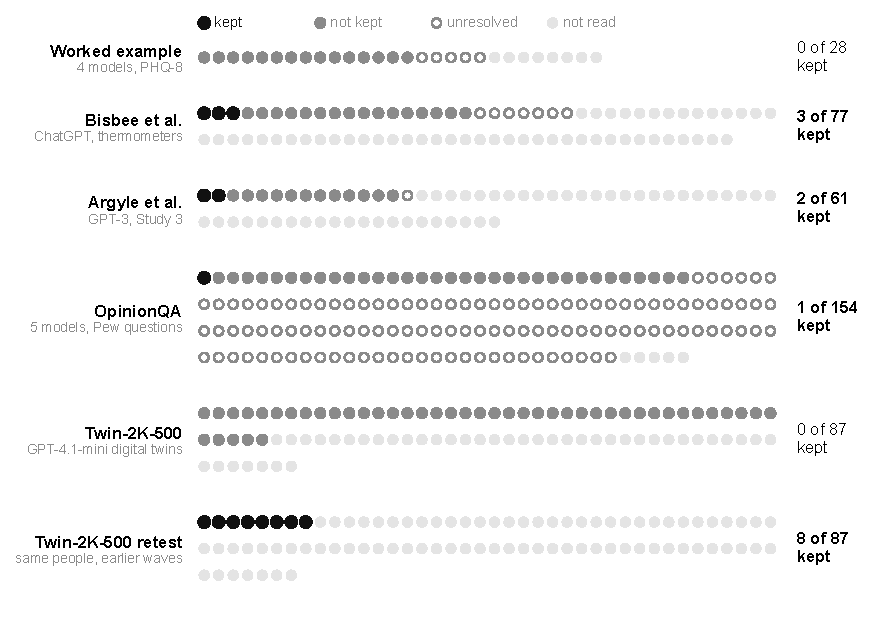
\includegraphics[width=\linewidth]{fig3_l2_dots.pdf}\par}
% Figure 3 note.
\figurenote{Each dot is one group gap, read per model in the worked example and OpinionQA and per thermometer or outcome in the releases of Bisbee et al.\ (full prompt), Argyle et al.\ (main run) and Twin-2K-500 (the authors' default twins).
A gap is kept when its interval lies between 0.75 and 1.25 times the real gap, not kept when it lies wholly outside that range, unresolved when it overlaps it, and not read when the reference cannot tell the gap from zero or measures it too imprecisely.
The two Twin-2K-500 rows show the 87 of 511 gaps whose human gap can be told from zero, and the retest row reads the same respondents' own answers from earlier waves as the simulator.
Intervals are Bonferroni-corrected within each model, prompt or run.} % R: ../../paper_brm/external/results/l2_threeway_summary.csv; ../../paper_brm/manuscript/figures/fig3_l2_dots_data.csv

\end{figure}
\FloatBarrier

% Written by paper_brm/external/harness/paper_table.py from results/CROSS_RELEASE.csv. Do not edit by hand.
\begin{table}[!ht]
\centering
\caption{Level-2 Readings of Released Simulators and of Faithful Controls}
\label{tab:external-all}
\footnotesize
\setlength{\tabcolsep}{3pt}
\resizebox{\linewidth}{!}{%
\begin{tabular}{@{}llrrrrrlrrrrr@{}}
\toprule
 & & \multicolumn{5}{c}{Simulators} & & \multicolumn{5}{c}{Faithful control} \\
\cmidrule(lr){3-7}\cmidrule(l){9-13}
Release & Simulator & $n$ & Pass & Fail & Unres. & Cannot & Control & $n$ & Pass & Fail & Unres. & Cannot \\
\midrule
\citet{bisbee2024synthetic} & ChatGPT & 3 & 0 & 3 & 0 & 0 &  & -- & -- & -- & -- & -- \\ % R: ../../paper_brm/external/harness/results/PAPER_TABLE.csv
\citet{argyle2023outofone} & GPT-3 & 3 & 0 & 3 & 0 & 0 & Ideal & 200 & 7 & 0 & 193 & 0 \\ % R: ../../paper_brm/external/harness/results/PAPER_TABLE.csv
\citet{meister2025distributional} & 5 LLMs & 26 & 0 & 13 & 12 & 1 & Ideal & 200 & 92 & 0 & 108 & 0 \\ % R: ../../paper_brm/external/harness/results/PAPER_TABLE.csv
\citet{huang2025uncertainty} & 8 LLMs & 8 & 0 & 7 & 1 & 0 & Ideal & 100 & 100 & 0 & 0 & 0 \\ % R: ../../paper_brm/external/harness/results/PAPER_TABLE.csv
 &  & -- & -- & -- & -- & -- & Ideal, small & 100 & 0 & 0 & 100 & 0 \\ % R: ../../paper_brm/external/harness/results/PAPER_TABLE.csv
\citet{suh2025subpop} & Base & 2 & 0 & 2 & 0 & 0 &  & -- & -- & -- & -- & -- \\ % R: ../../paper_brm/external/harness/results/PAPER_TABLE.csv
 & SubPOP & 2 & 0 & 2 & 0 & 0 &  & -- & -- & -- & -- & -- \\ % R: ../../paper_brm/external/harness/results/PAPER_TABLE.csv
\citet{toubia2025twin2k} & 13 twins & 13 & 0 & 13 & 0 & 0 & Retest & 1 & 1 & 0 & 0 & 0 \\ % R: ../../paper_brm/external/harness/results/PAPER_TABLE.csv
\citet{peng2025funhouse} & 23 twins & 413 & 0 & 285 & 0 & 128 & Split half & 18 & 0 & 0 & 0 & 18 \\ % R: ../../paper_brm/external/harness/results/PAPER_TABLE.csv
\citet{malmberg2026conjoint} & 3 LLMs & 3 & 0 & 2 & 0 & 1 & Split half & 3 & 0 & 0 & 0 & 3 \\ % R: ../../paper_brm/external/harness/results/PAPER_TABLE.csv
\citet{cummins2026flexibility} & 9 LLMs & 252 & 0 & 0 & 0 & 252 & Split half & 200 & 0 & 10 & 0 & 190 \\ % R: ../../paper_brm/external/harness/results/PAPER_TABLE.csv
\midrule
All simulators & & 725 & 0 & 330 & 13 & 382 & & & & & & \\ % R: ../../paper_brm/external/harness/results/PAPER_TABLE.csv
\bottomrule
\end{tabular}}
\vspace{4pt}
\begin{tabnote}
\textit{Note.} Each reading is one family of contrasts read together, such as one model under one prompt (one model and study for \citet{peng2025funhouse}). Pass: every contrast read is kept. Fail: at least one is not kept. Unres.: neither, with at least one contrast the reference could certify. Cannot: none is not kept, and the reference could not certify a kept verdict on any contrast in the family (step 0). Simulators: ChatGPT under 3 prompts; GPT-3 in 3 runs; 5 LLMs under 3 elicitation and 2 steering methods; Mistral-7B before (Base) and after (SubPOP) survey training; twin specifications, over 18 studies for \citet{peng2025funhouse}; 252 configurations of 9 LLMs. Ideal: a fresh sample of the released human answers at the human group sizes; Ideal, small: the same at the size of the LLM samples. Retest: the respondents' own answers in earlier waves. Split half: one half of the respondents read against the other. \citet{suh2025subpop} is read against SubPOP's processed copy of the human answers to the questions of \citet{meister2025distributional}, whose ideal simulator is the nearest control (Supplement S8).
\end{tabnote}
\end{table}


Where a release gives only answer distributions or a small panel, the reference decides much of the verdict.
\citet{meister2025distributional} released the answer distributions of five models steered toward demographic groups on OpinionQA questions \citep{santurkar2023whose}, beside Pew's distributions for the same groups.
With no individual respondents the reference gives only crude gaps, and the ladder leaves most contrasts unresolved where a comparison of point estimates would have credited 37 of them as matching. % R: ../../paper_brm/external/results/l2_threeway_summary.csv; ../../paper_brm/external/results/l2_threeway_rows.csv
Seven of the eight LLMs in \citet{huang2025uncertainty} fail, and a fresh sample of the human answers passes at the human group sizes and is unresolved at the size of the LLM samples. % R: ../../paper_brm/external/harness/results/PAPER_TABLE.csv
Two of the three LLMs making conjoint choices in \citet{malmberg2026conjoint} fail, and the reference cannot certify the third. % R: ../../paper_brm/external/harness/results/PAPER_TABLE.csv
In the multiverse of \citet{cummins2026flexibility}, 252 LLM configurations answer for at most 85 people per contrast, and step 0 reports that reference as unable to certify any of them. % R: ../../paper_brm/external/harness/results/DESIGN.csv; ../../paper_brm/external/harness/results/PAPER_TABLE.csv
Whether a pass is reachable depends on the precision of the reference and the size of the sample as well as on the simulator.

SubPOP \citep{suh2025subpop} is the one simulator in the set trained to reproduce subgroup answers, Mistral-7B \citep{jiang2023mistral} fine-tuned on Pew and General Social Survey subgroup distributions, which we ran beside its base model on the OpinionQA questions of \citet{meister2025distributional}.
Its base model shows almost no group structure, and after training every gap points in the human direction, seven of eight at 0.30 to 0.56 of the human size, with no gap kept (Supplement S8). % R: ../../paper_brm/external/harness/results/DESIGN.csv; ../../paper_brm/external/harness/results/subpop2025/l2_contrasts.csv
None of these questions appears in SubPOP's released training data, although four are items that the training data carry from another survey wave. % R: ../../paper_brm/external/harness/results/subpop2025/training_overlap.csv
Readings without those four, or without the questions fielded during the training period, give the same pattern (Supplement S8). % R: ../../paper_brm/external/harness/results/subpop2025/l2_contrasts_no_overlap.csv; ../../paper_brm/external/harness/results/DESIGN.csv
Training on subgroup answers corrected the direction of the gaps and left their size short of people's.

The personality release \citep{ipipaudit2026} holds 10,000 answers from each of eight current LLMs to the 50 IPIP Big Five markers, beside 500,703 human respondents. % R: ../../paper_brm/explore_2026-10-03/personality/out/p23_paper_numbers.csv
Every model fails level 1 on every scale with too few unusual answer patterns, and every model's item loadings differ from people's (R2), while 10,000 held-out people pass both. % R: ../../paper_brm/explore_2026-10-03/personality/out/p23_paper_numbers.csv

Two exploratory analyses, one on the PHQ-8 corpus and one on the default twins, ask why the simulated gaps go wrong (Supplement S8).
In the corpus, income carries most of the variance among the models' persona means (.79 to .90, against .33 in NHANES), a weighting no linear recalibration removes. % R: ../../paper_brm/explore_2026-10-03/mechanism_corpus/A_main_effect_shares.csv; ../../paper_brm/explore_2026-10-03/mechanism_corpus/B_halfsplit_summary.csv
In the default twins, party carries far more of the partisan gap than it does in people. % R: ../../paper_brm/explore_2026-10-03/mechanism_twins/B_pooled.csv
In both, one persona attribute carries more of the simulated answer than it carries in people.

% Section 6. Discussion and conclusion. Built from Patrick's spoken answers (4 Oct 2026); conceptual, results stay in Sections 3-5.

\section{Discussion}
\label{sec:discussion}

Researchers who use LLM-simulated populations need to validate each claim they draw from them with the same rigor they would apply to a new human measure, and the ladder supplies a structure for doing so.
A persona sample can be used to report group gaps, population levels, single cases or scale scores, and each of these uses is a separate extrapolation from the model's answers.
The failures found in the worked example sat at these separate uses and could not be seen in any single answer or in a correlation of group means.
In practice each claim is checked against the rung built to test it, with the model's ability to stand in for people held in critical doubt until that check is passed.

The ladder asks for its human reference before anything is generated.
Every rung above the gate reads the simulated sample against human answers to the same instrument, and a study without that reference cannot use it.
Because the reference sets which personas can be compared, how many draws each persona needs and which gaps can be certified, step 0 reads the reference on its own and returns the gaps on which a pass is reachable for any simulator.
With that list in hand a researcher either enlarges the reference or narrows the claims the study will make.
The mapping of each persona attribute to a reference variable is fixed at the same point and reported beside the verdicts, as the dollar amount on the income label and the poverty-ratio band gave different verdicts on the low-to-high income contrast for two models in the worked example. % R: l2_verdicts.csv
Personas drawn from real respondents' profiles, the design \citet{bisbee2024synthetic} and \citet{argyle2023outofone} used, give every simulated answer a human counterpart and the cleanest reference available.

Across the external releases, current models often fell short as simulated populations.
None of the samples read at level 2 passed it, and in many releases the human reference itself limited which gaps could be tested.
\citet{bisbee2024synthetic} and \citet{argyle2023outofone} reported algorithmic fidelity, and the ladder supports the partisan gaps in their samples while most gaps by sex, age and race fail or go unread.
The verdicts give a narrower reading of their claims of fidelity and leave their findings in place.
Twin-2K-500 separates two properties that are easily treated as one, since digital twins that matched many individual answers still distorted the partisan gaps while the respondents' own earlier answers passed. % R: ../../paper_brm/external/results/twin2k/summary.csv
We read the comparison as evidence that a twin's accuracy on individual answers does not carry over to the gaps between groups.

Training on subgroup survey answers moved a model in the right direction.
The base model of SubPOP showed almost no group structure, and after fine-tuning every gap pointed the way the human gap points, short of the human size and without a pass.
We read the result as promising and as pointing toward the interventions these models need before they can be relied on, while current training remains insufficient for a study to skip the checks.
We do not read it as a ceiling on what training can do, and a fine-tuned simulator goes through the same rungs as any other.
\citet{hullman2026validating} and \citet{wang2026substitutability} pursue the same tie to human data in concurrent work, calibrating simulated effects against auxiliary human samples and asking how far digital twins can substitute for human measurement of a given estimand.

The controls give the grounds for trusting the verdicts.
Samples built from real respondents rarely fail, failures planted into those respondents are caught at the rung each targets, and faithful controls in the external releases pass wherever the reference can certify a gap.
Relaxing the rules does not rescue the models, as wider kept regions and an uncorrected test leave almost every simulator reading failed or unresolved (Supplements S4.7 and S8).

The thresholds given with each rung are defaults.
Tolerance is set by the user, who reads the verdicts against the level of risk the application carries and chooses a kept region accordingly.
A pilot or exploratory study can set a looser tolerance than a study whose results will inform decisions about people, and we make no claim about the tolerance any study must hold.
The ladder is built to be adapted to a study's needs and applied where its requirements are met.

Several limits remain.
Under designs like the worked example's, with a few dozen draws per persona and a national survey as reference, many group gaps go unresolved or unread, and an unresolved verdict can reflect the design as much as the simulator.
The worked example also gives each demographic cell a single persona with no stated age, one wording per attribute and the items in one order, and its verdicts hold for that design.
Level 4 has no certifiability step, and a faithful sample can fail it by chance where the reference lies near a threshold (Supplement S8).
As specified, the ladder does not read contrasts with no population gap, leaving untested any gap a model invents where people show none, a case the exploratory equivalence test in Supplement S4 begins to address.
Finally, every rung depends on a human reference on the same instrument, and where none exists the ladder cannot certify a simulated population for any use.

\subsection*{Conclusion}

The validity ladder replaces a single judgment of whether a simulated sample resembles people with a separate check for each use of the sample, each carrying a pass rule, a human reference and the claim it supports.
Judging a simulated sample by how plausible its answers look is not enough, and every model in the worked example would have passed that judgment.
A claim about a simulated population becomes specific to one use and checkable against people, and the human reference becomes the constraint a study plans and budgets for before it generates anything.
As fine-tuning and grounding improve, a common set of checks gives a way to measure how far simulated populations have come.
We release the code for every rung and the receipt for every number, allowing grounded or fine-tuned simulators to be checked against the same baseline.

% 08_limitations folded into the Discussion in the 2 Oct 2026 rewrite.
% Declarations, AI statement and Open Practices Statement (BRM). The Open Practices Statement
% must sit immediately before the References, so it is last here. Headings follow the BRM
% submission guidelines (Declarations list; Open Practices section), checked 4 Oct 2026.

\section*{Declarations}

\paragraph{Funding.} No funding was received for this work.

\paragraph{Competing interests.} The author has no competing interests to declare.

\paragraph{Ethics approval.} Not applicable. The study analyzes public, de-identified NHANES microdata, released data from other studies and text generated by language models. No human participants were recruited.

\paragraph{Consent to participate.} Not applicable.

\paragraph{Consent for publication.} Not applicable.

\paragraph{Availability of data and materials.} The corpus, the persona registries, the original generation code for both framings, the outputs of every analysis and every receipt file are at \url{https://github.com/pskeough/A-Validity-Ladder-for-LLM-Simulated-Populations}. NHANES data are public from the National Center for Health Statistics, and the repository includes the code that extracts them. Raw files of the external releases are not redistributed, and the repository names the public source of each. SubPOP's training data, used only to check question overlap, derive from Pew Research Center's American Trends Panel and the General Social Survey \citep{davern2024gss}. The opinions expressed herein, including any implications for policy, are those of the author and not of the survey research centers.

\paragraph{Code availability.} The analysis scripts are in the same repository. Every level-2 external release can be read through \texttt{paper\_brm/external/harness}, whose self-test reproduces the verdicts of the article's own scripts on 14,349 stored contrasts with no mismatch, and the personality release was read through the article's level-1 and level-4 code. The Python package \texttt{validity-ladder} (version 0.1.1) implements the gate, levels 1 to 4 and step 0, taking the invariance verdict R4 as an input. It installs with \texttt{pip} and carries tests that reproduce the article's verdicts from the stored outputs.

\paragraph{Authors' contributions.} Patrick Keough is the sole author and takes responsibility for all content.

\paragraph{Generative AI disclosure.} Generative AI tools (Anthropic's Claude, through Claude Code) were used for language editing, for LaTeX formatting, and to write the Python analysis and verification scripts to the author's specification. The research questions, study design, statistical specification and interpretations are the author's own, and all generated code was reviewed by the author. The verification scripts that check every numeric claim in this manuscript against its receipt are released with the data.

\section*{Open Practices Statement}

Data, materials and analysis code are available at \url{https://github.com/pskeough/A-Validity-Ladder-for-LLM-Simulated-Populations}, release commit \texttt{COMMIT}, where \texttt{paper\_brm/manuscript/supplement/S2\_receipts.csv} maps every number in the article to the file that prints it. None of the analyses were preregistered.


\bibliography{refs}

\end{document}
